\chapter{Spearman Alignment Charts (Studies 07--10)}
\label{appendix:spearman-charts}

This appendix collects the \texttt{spearman\_chart.png} bar plots produced by the evaluation harness for Studies~07--10 
(Section~\ref{sec:human-machine-alignment}). Spearman coefficients, $p$-values, 
and discussion appear in the main evaluation chapter. The charts are provided here for reference, and to minimise 
the clutter of the main text.

This appendix serves as visual representation of the Spearman rank correlation coefficients for the four studies (Studies 07-10).
The charts are provided here for reference, with tables being provided in 
Table~\ref{tab:spearman-study-07}, 
Table~\ref{tab:spearman-study-08}, 
Table~\ref{tab:spearman-study-09}, 
and Table~\ref{tab:spearman-study-10}.


\begin{figure}[htbp]
    \centering
    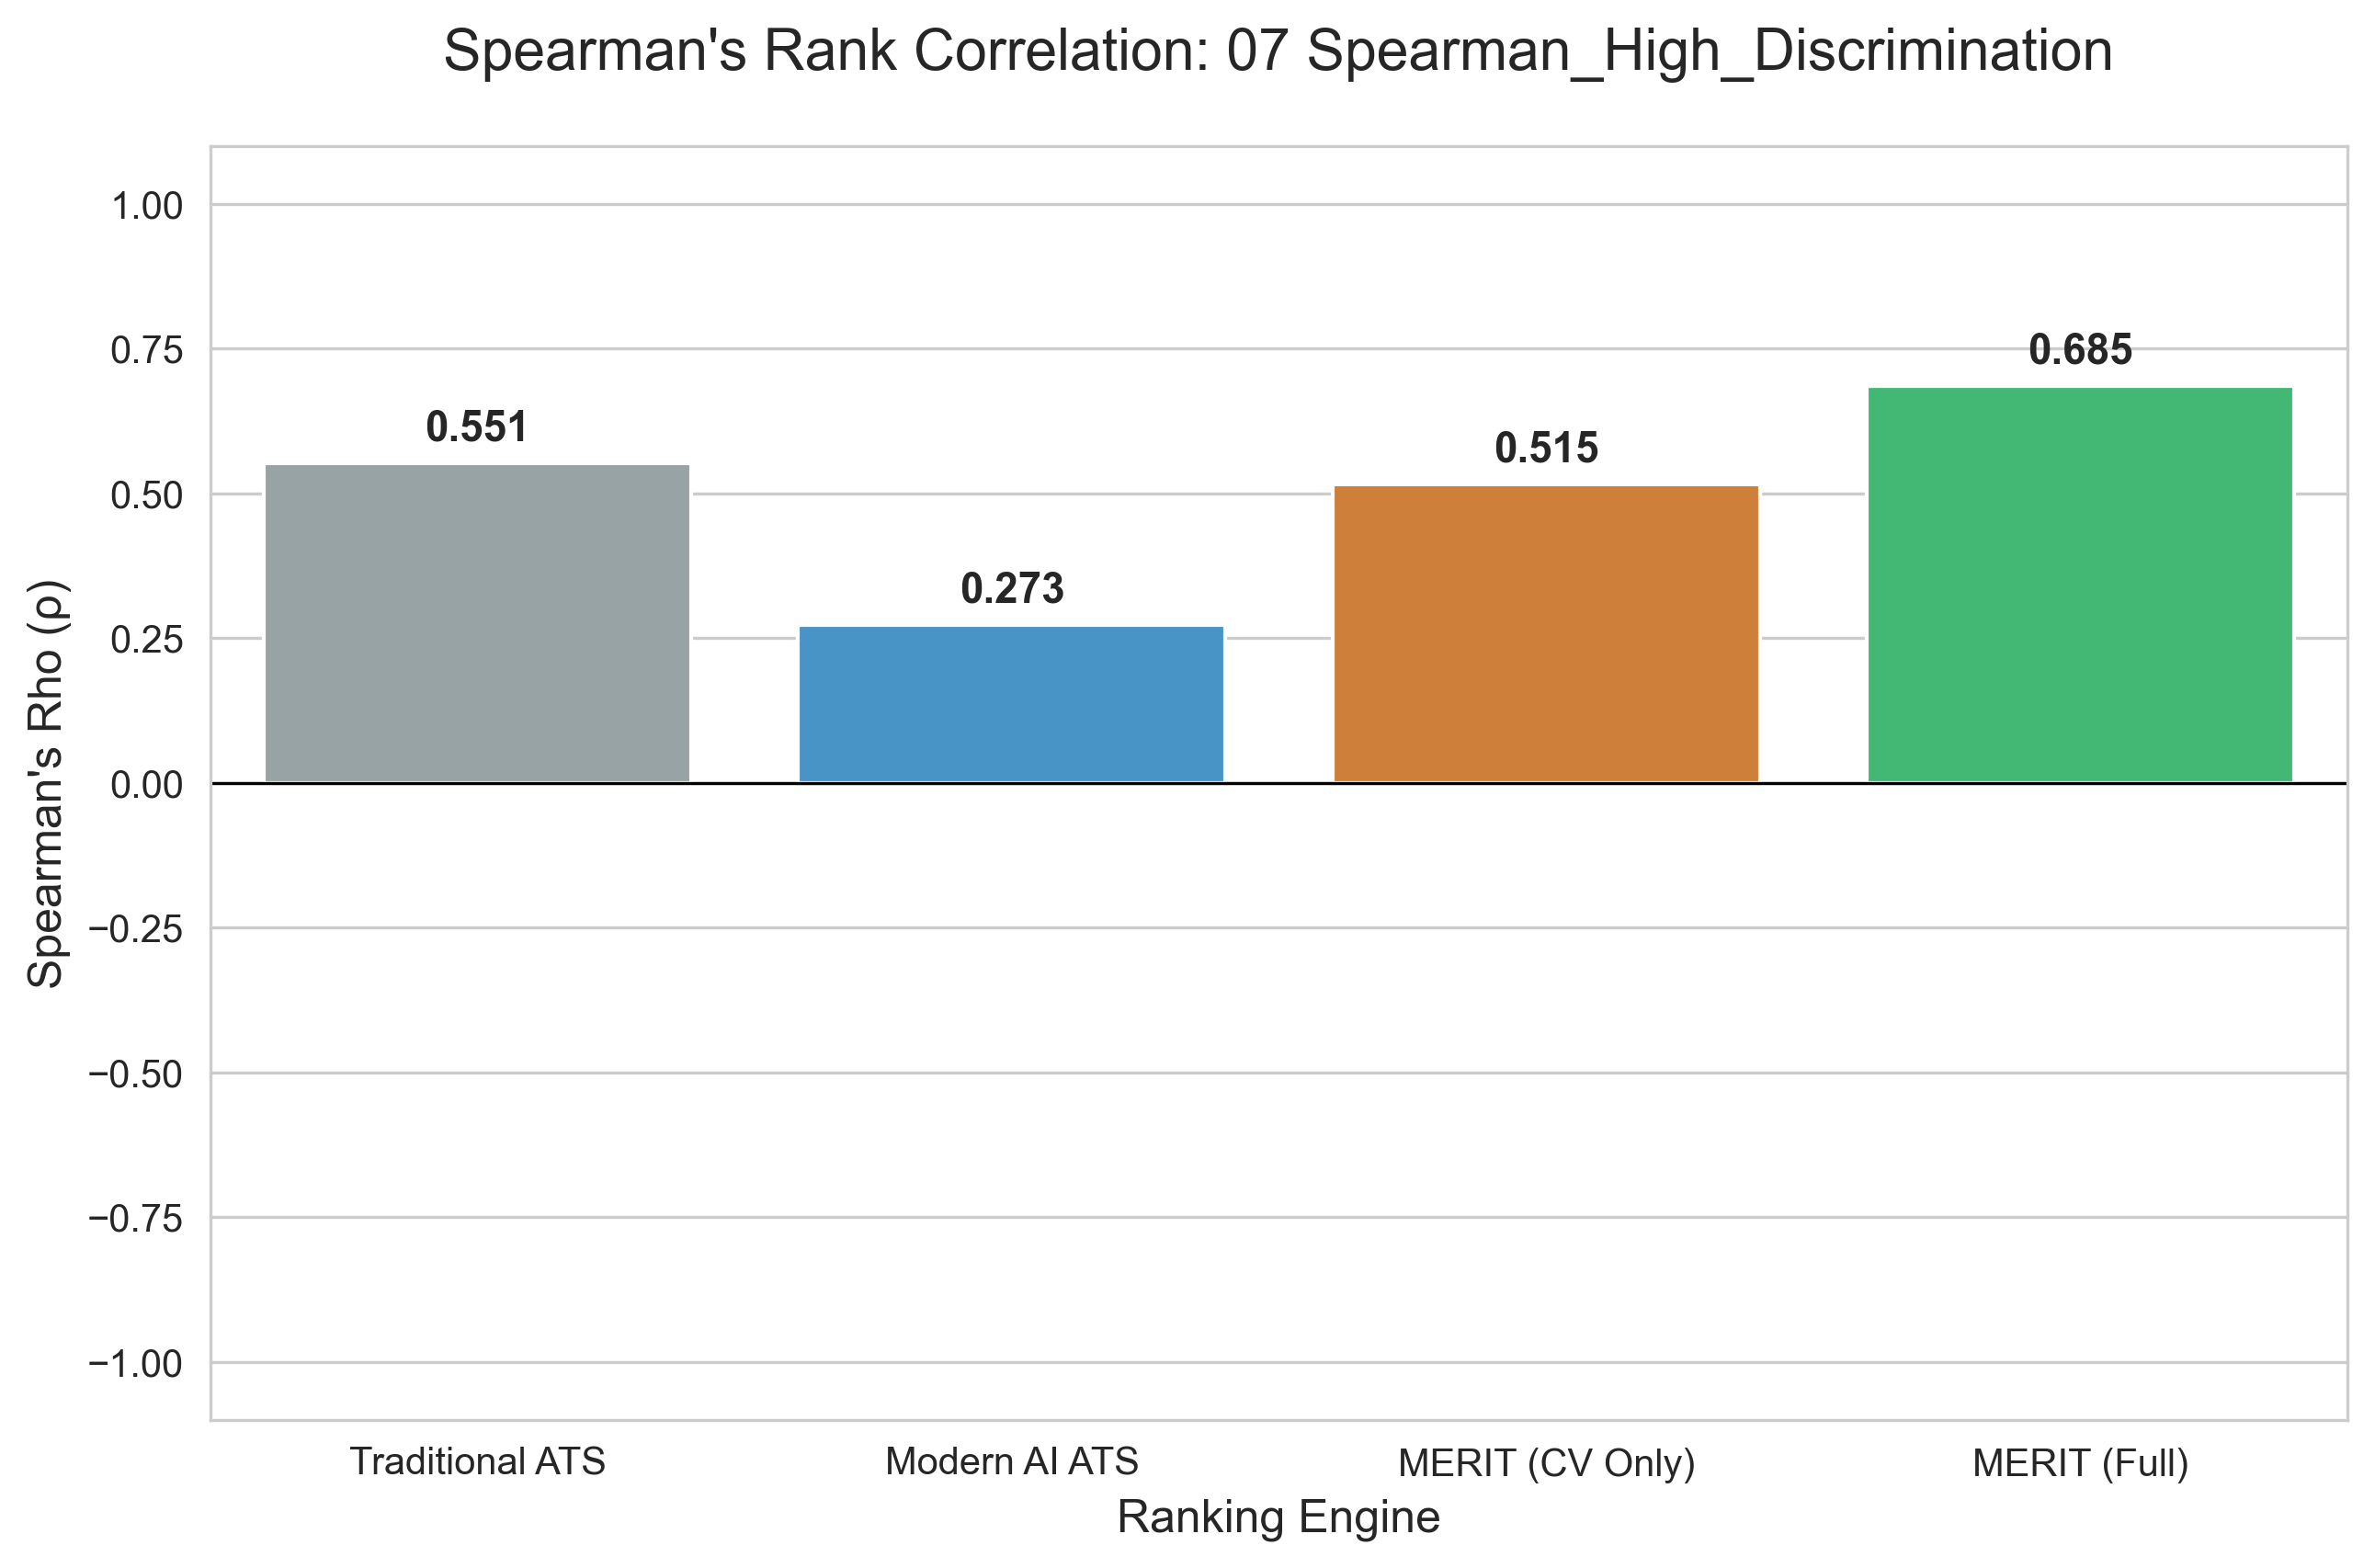
\includegraphics[width=0.92\textwidth]{../evaluation/07-spearman_high_discrimination/output/spearman_chart.png}
    \caption[Study~07: Spearman $\rho$ by engine (high discrimination)]{Study~07: Spearman $\rho$ by engine for 
    the high discrimination cohort. MERIT (Full) attains the highest bar, with baseline models exhibiting weaker alignment.
    These results are tabulated in Table~\ref{tab:spearman-study-07}.}
    \label{fig:spearman-study-07}
\end{figure}

\begin{figure}[htbp]
    \centering
    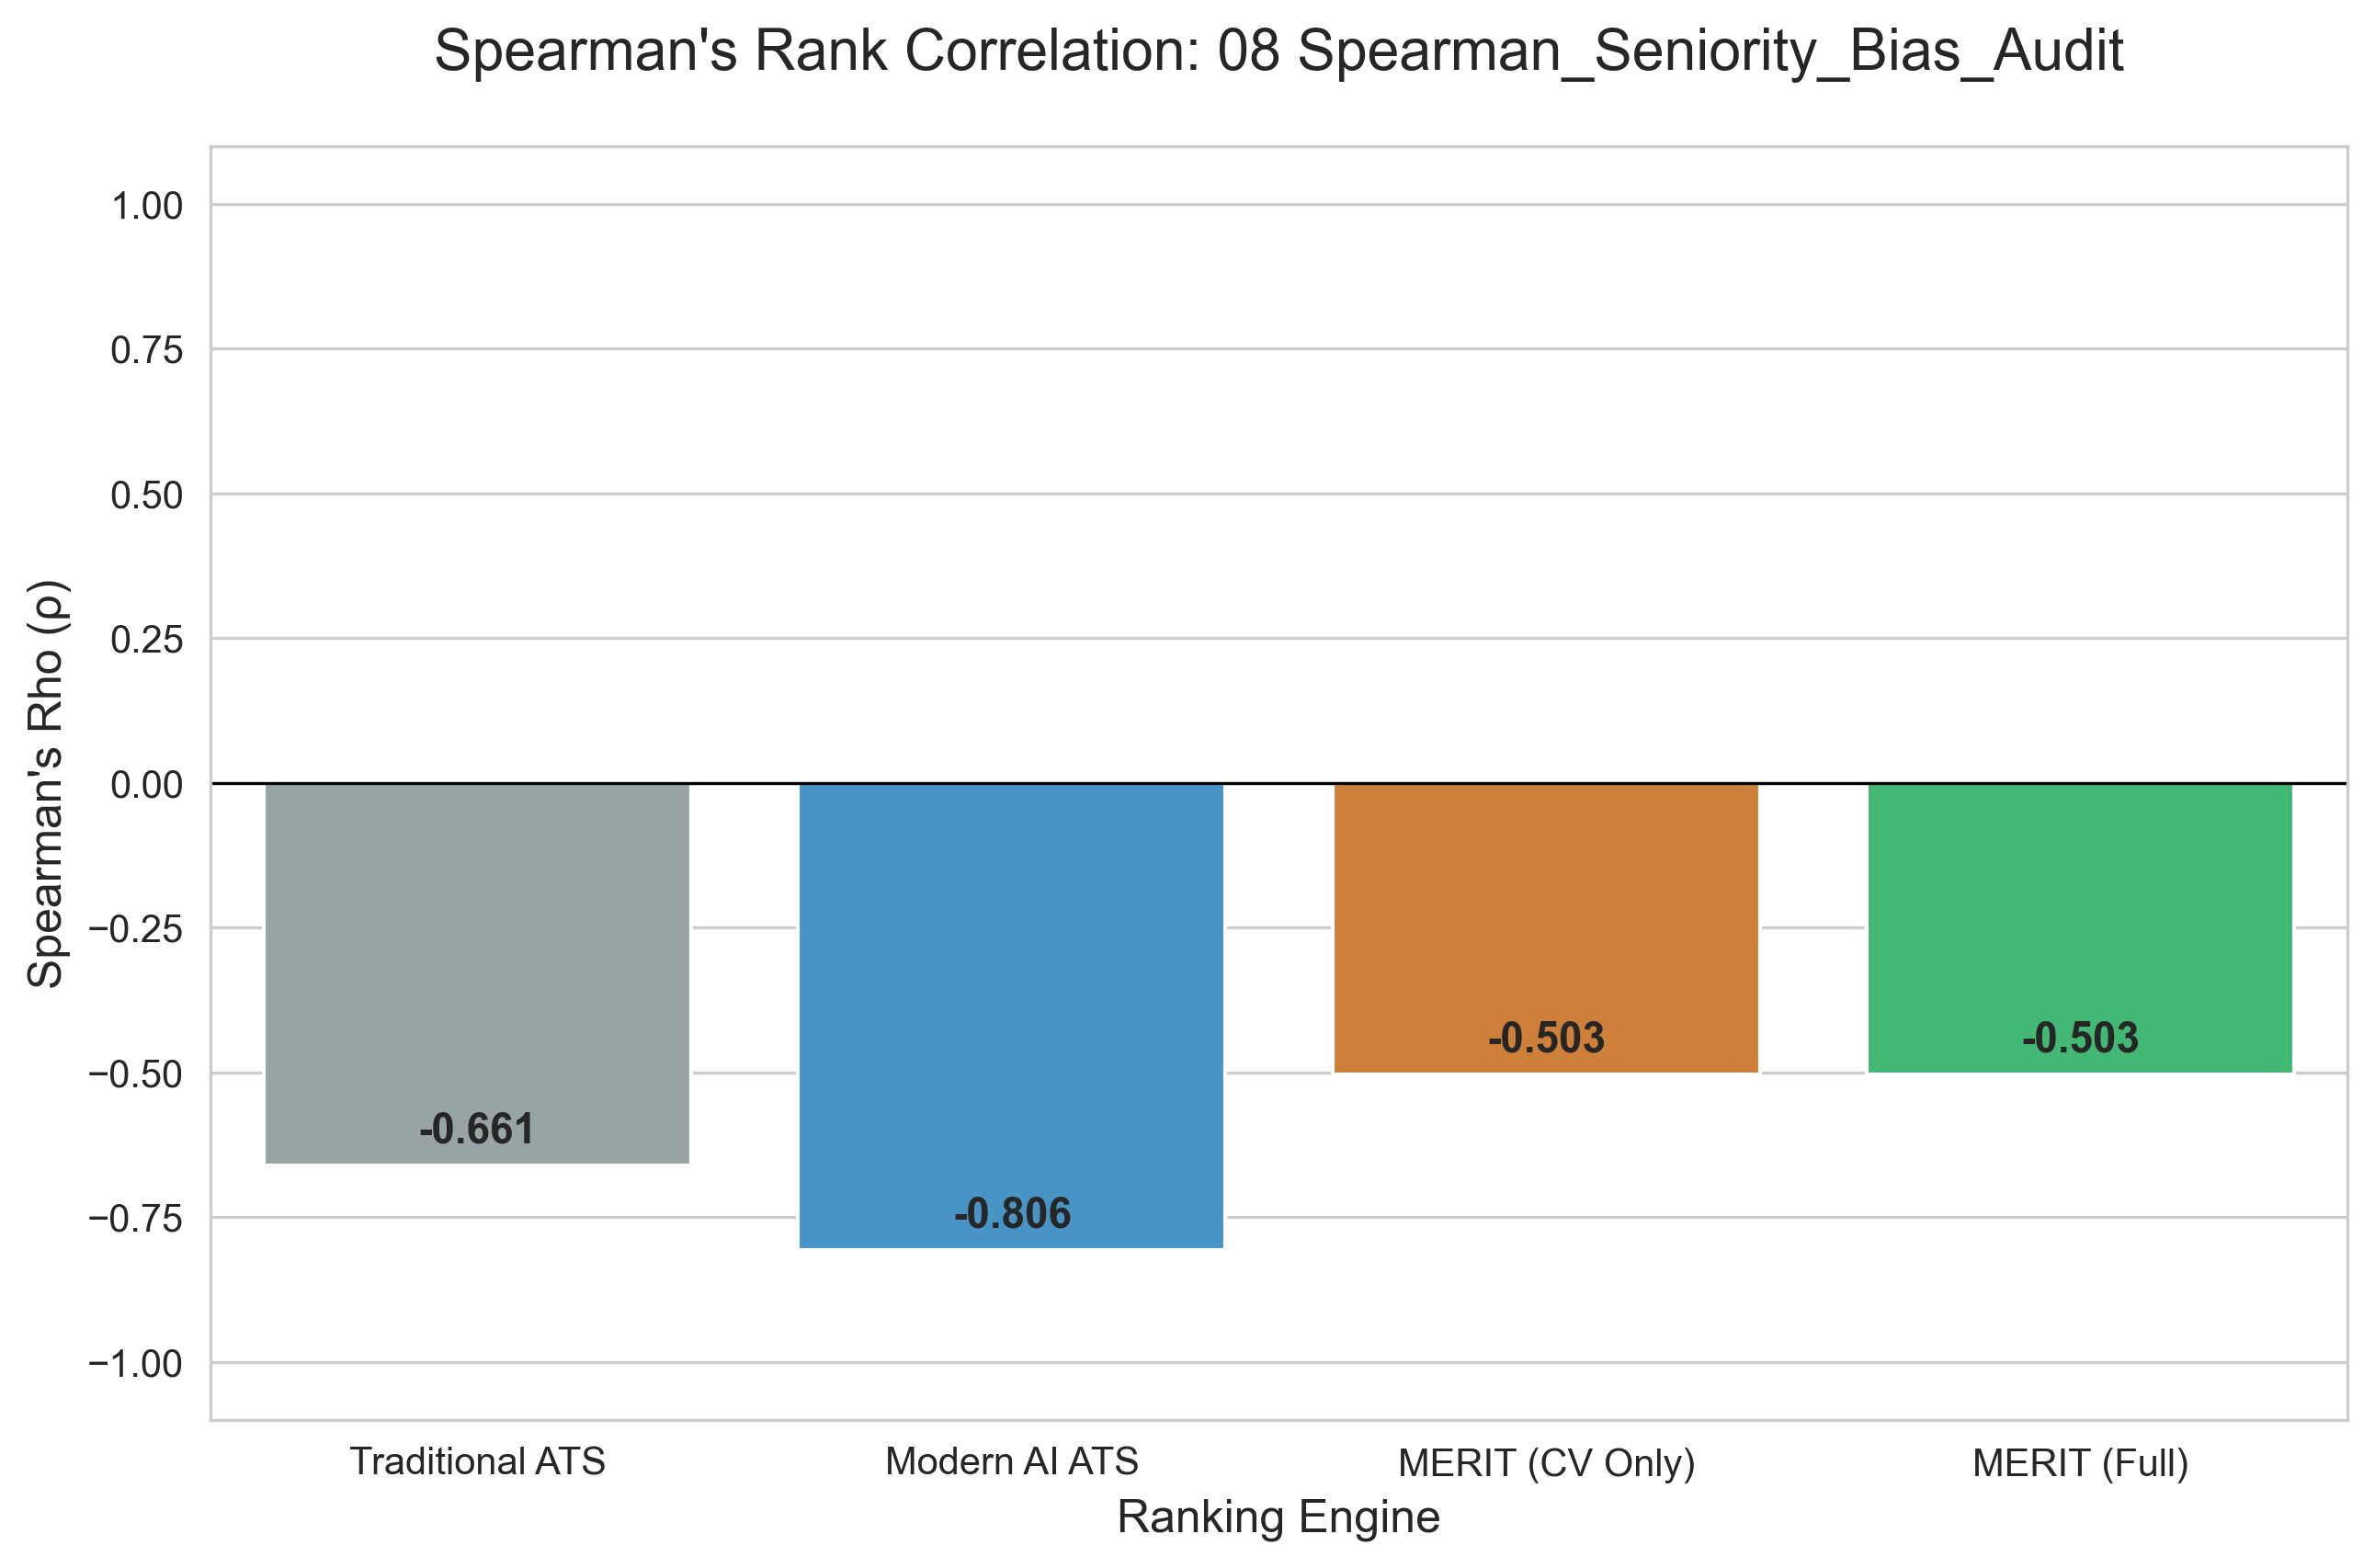
\includegraphics[width=0.92\textwidth]{../evaluation/08-spearman_seniority_bias_audit/output/spearman_chart.png}
    \caption[Study~08: Spearman $\rho$ by engine (seniority-bias audit)]{Study~08: Spearman $\rho$ by engine for the 
    seniority-bias cohort. All engines are significantly anti-aligned with the expert consensus, due to preferring
    candidates with the highest seniority, rather than the human preferred "best fit" for a low-experience role.
    Note that all ATS systems fail to understand the concept of overqualified candidates.
    Note that MERIT (Full) remains negatively correleted, but less extreme than the other two, non-MERIT baselines.
    This is due to the design of MERIT prioritising the quality of the evidence over the seniority of the candidate.
    These results are tabulated in Table~\ref{tab:spearman-study-08}.}
    \label{fig:spearman-study-08}
\end{figure}

\begin{figure}[htbp]
    \centering
    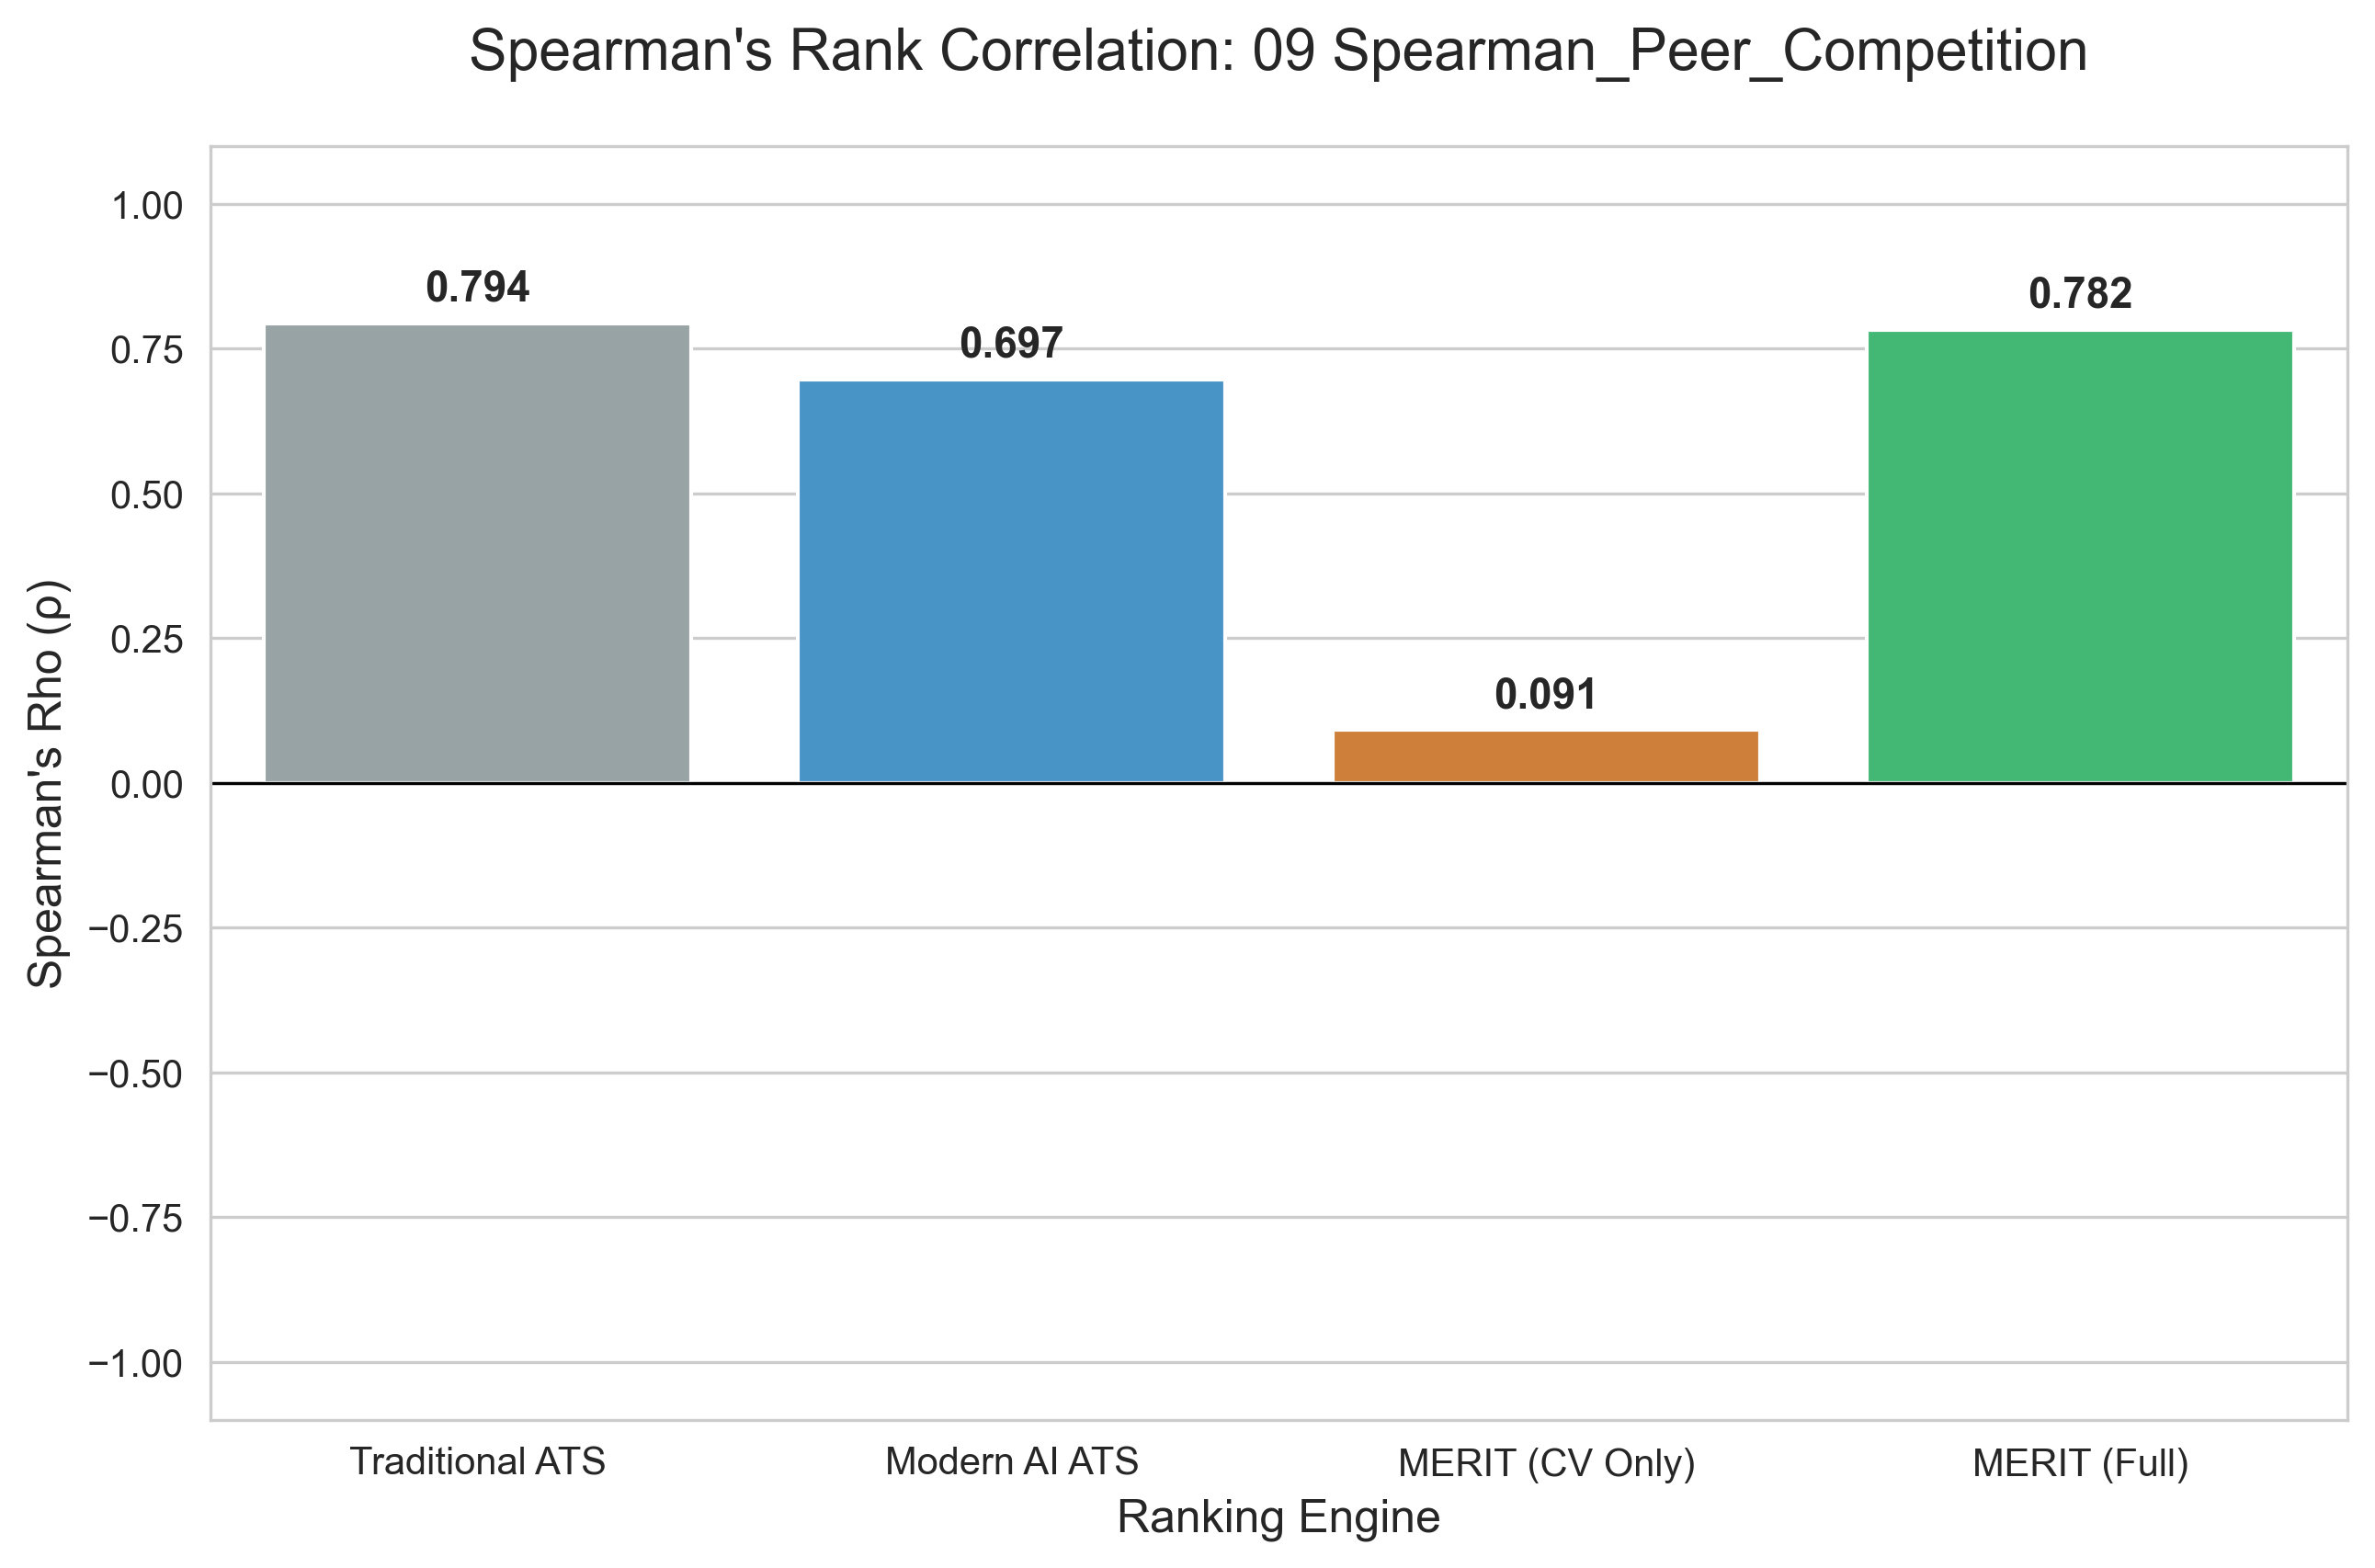
\includegraphics[width=0.92\textwidth]{../evaluation/09-spearman_peer_competition/output/spearman_chart.png}
    \caption[Study~09: Spearman $\rho$ by engine (peer competition)]{Study~09: Spearman $\rho$ by engine for the 
    peer competition cohort. The traditional ATS is most correlated with this particular expert ordering,
    while MERIT (Full) is able to achieve a relatively strong alignment with the expert consensus.
    These results are tabulated in Table~\ref{tab:spearman-study-09}.}
    \label{fig:spearman-study-09}
\end{figure}

\begin{figure}[htbp]
    \centering
    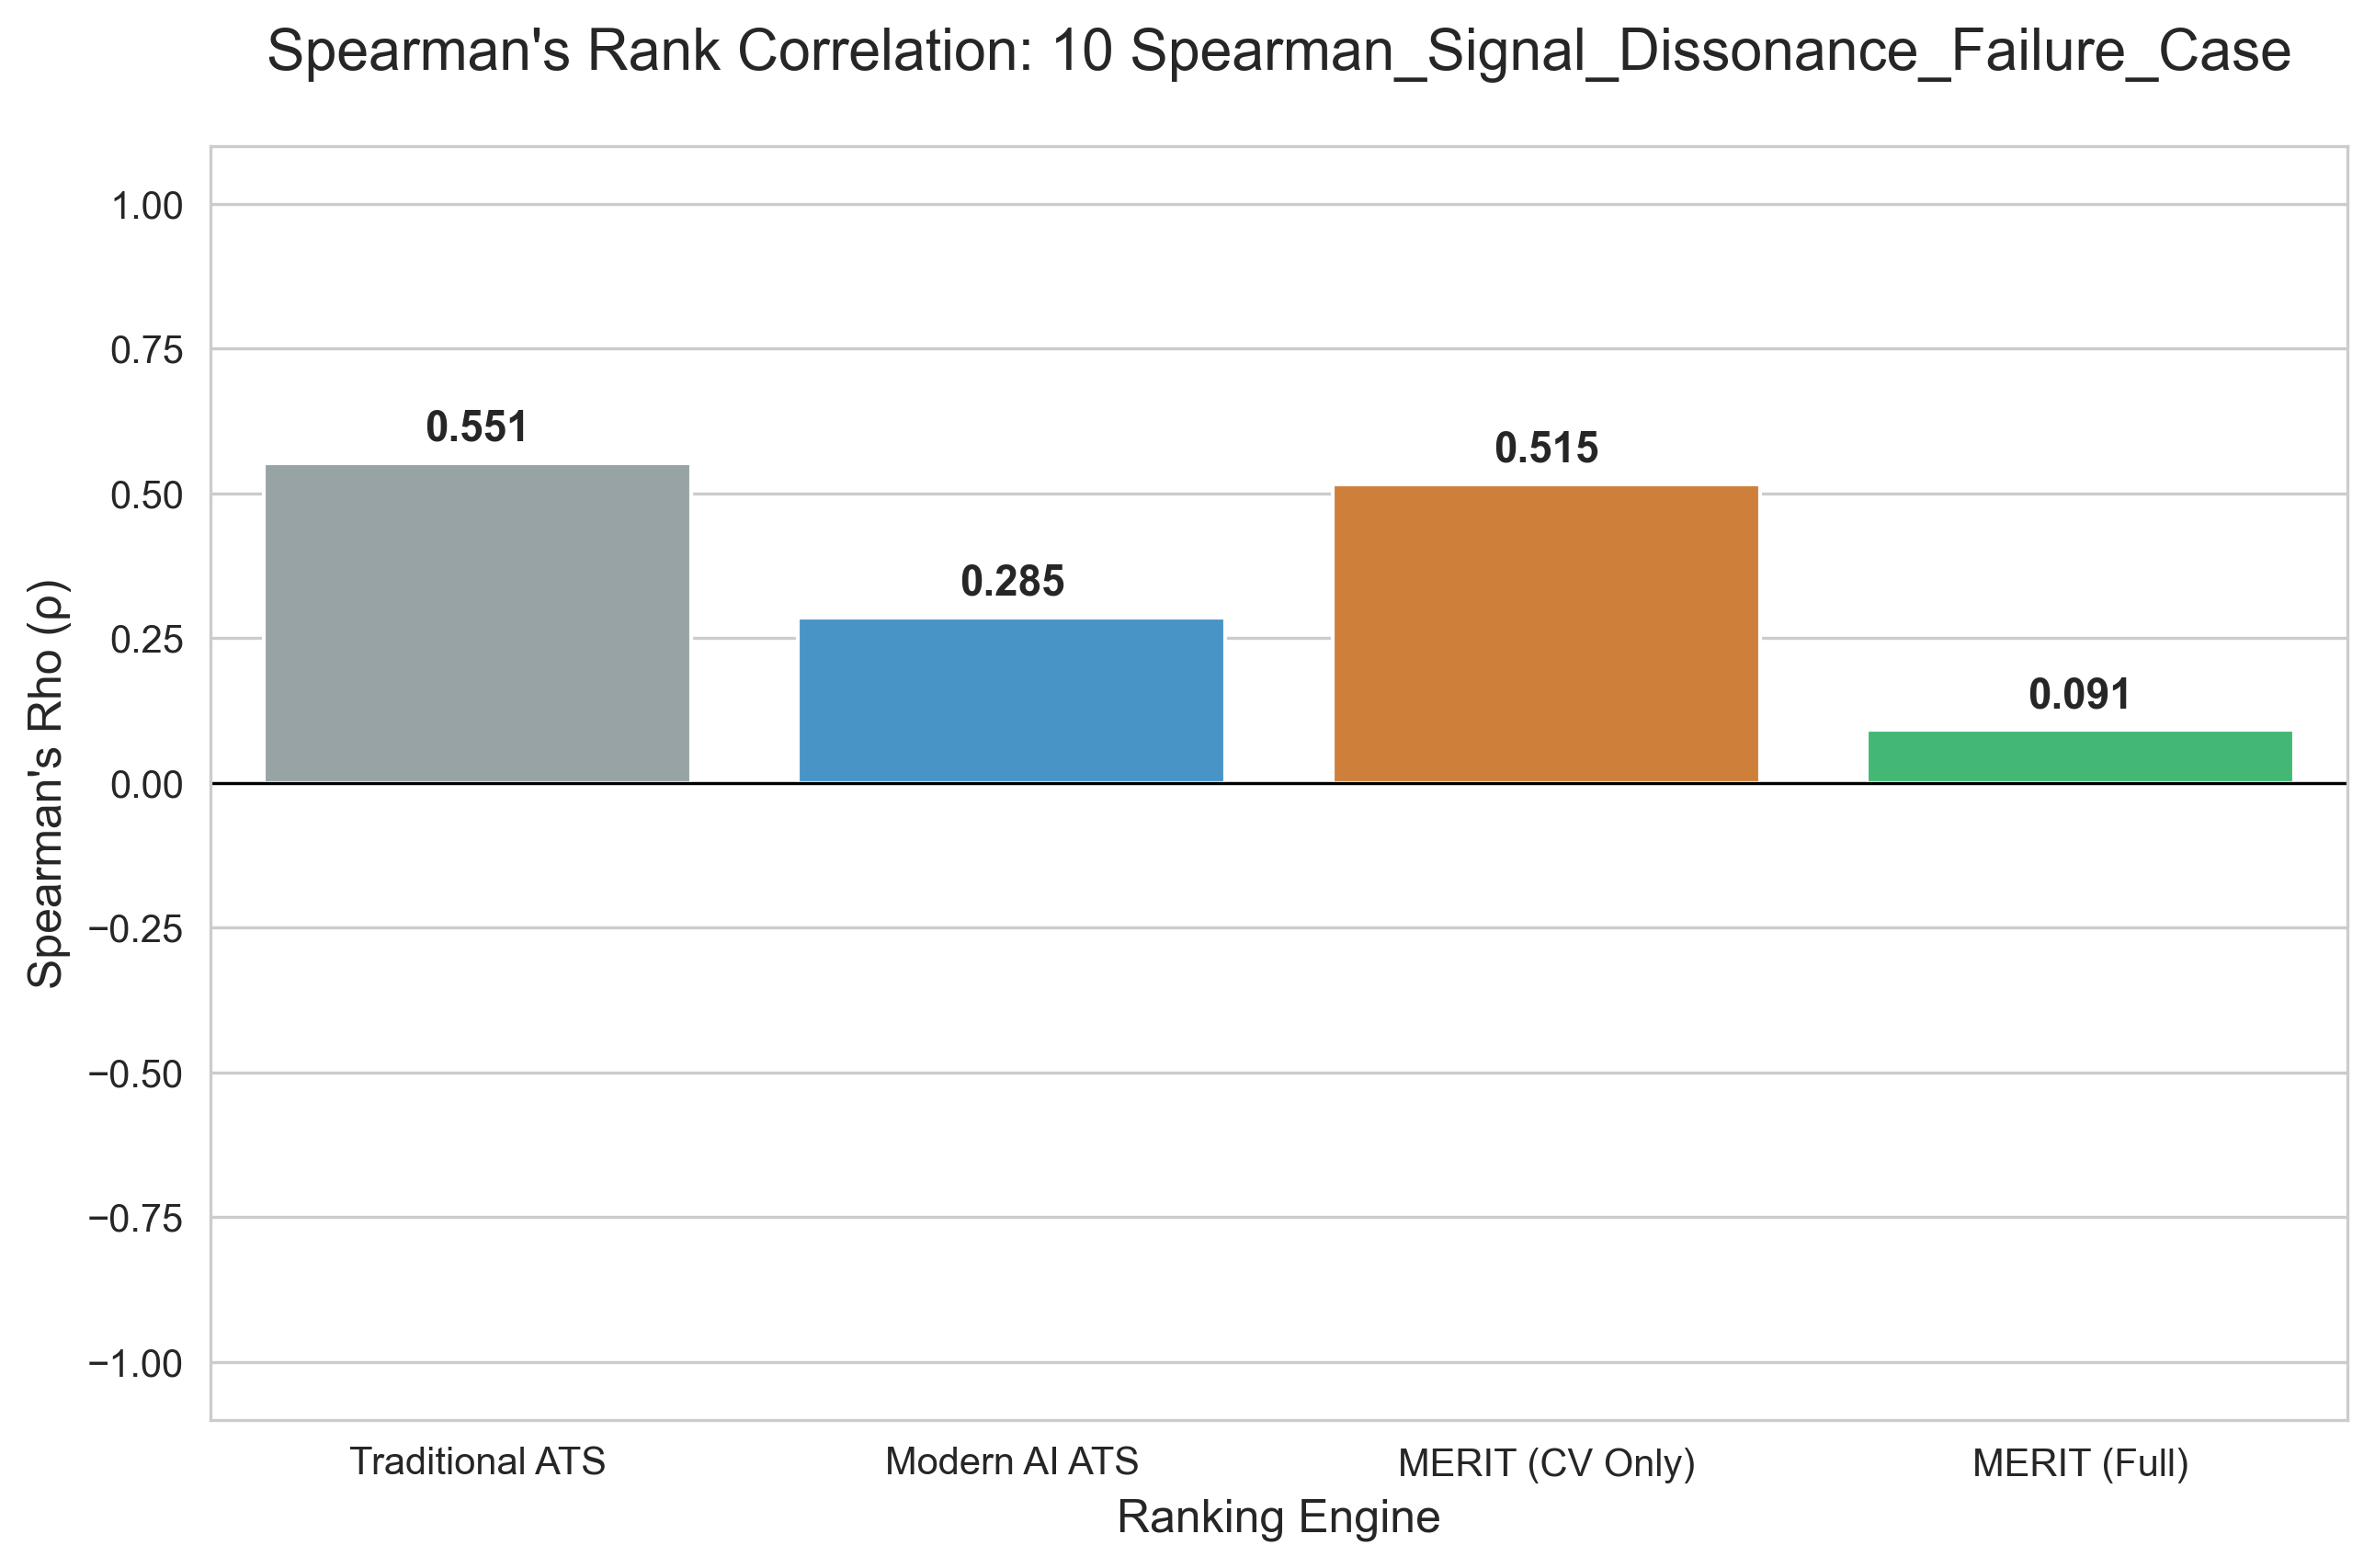
\includegraphics[width=0.92\textwidth]{../evaluation/10-spearman_signal_dissonance_failure_case/output/spearman_chart.png}
    \caption[Study~10: Spearman $\rho$ by engine (signal dissonance)]{Study~10: Spearman $\rho$ by engine for the 
    signal dissonance cohort. The MERIT (Full) bar collapses toward zero, visualising the failure of MERIT (Full) 
    to correctly rank the candidates when the data sources are contradictory. Note that this is not a real-world
    scenario, but rather a deliberate failure case to highlight the vulnerability of MERIT (Full) to contradictory evidence.
    In a real-world scenario, the majority of candidates would not have significantly contradictory evidence between the CV 
    and external evidence. This is a key finding that highlights the importance of the quality of the evidence when using multi-source fusion.
    These results are tabulated in Table~\ref{tab:spearman-study-10}.}
    \label{fig:spearman-study-10}
\end{figure}
